From the previous section we can see that, the unbiased estimated decision value of LOO-CV for an example can be written in a closed form. In this section, we introduce the multi-class loss function and use the LOO-CV error to estimate the multi-class loss. We propose a novel objective function based on the estimated multi-class loss to estimate the transfer parameters.

In previous section, we discussed the LS-SVM in binary class scenario. In practice, we have to handle the multi-class scenario. A common strategy to convert the binary class scenario to a multi-class scenario is to assign label to the highest confidence score of each binary SVM. Suppose we trained $n$ binary SVMs $f_i,i\in 1,...,n$ for a $n$-class problem, the label of an example $x$ is assigned by:
\begin{figure}
	\centering
	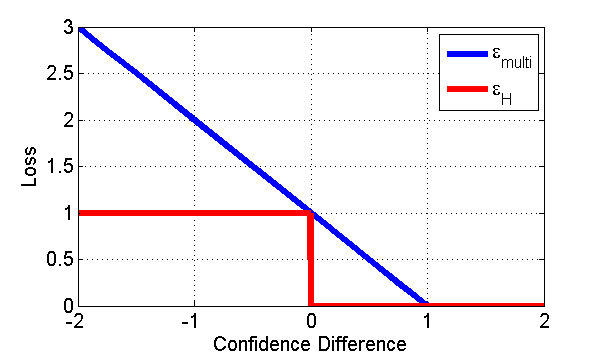
\includegraphics[scale=.7]{transfer/fig/losscmp.png}
	\caption{Loss function comparision for multi-class hinge loss $\epsilon_{multi}$ and classical zero-one loss  $\epsilon_{H}$}\label{fig:single:losscmp}
\end{figure}
\begin{equation}
H_{\mathcal{F}}(x)=\hat{y}=\arg \underset{i \in 1,...,n}{\max}f_i(x)
\end{equation} 
Let $\llbracket y\rrbracket$ be 1 if the predicate $y$ holds and 0 otherwise. The empirical error for a multi-class problem is given by:

\begin{equation} \label{eq:single:discreteloss}
	\epsilon_{H} = \frac{1}{l}\sum_{1}^{l}\llbracket H_{\mathcal{F}}(x_i) \neq y_i \rrbracket
\end{equation}
Our goal is to find a group of function $\mathcal{F}$ that has a small empirical error on the training set as well as on an unforeseen test set. Because function \eqref{eq:single:discreteloss} takes discrete value on the predicate, directly approaches which tries to minimize the empirical error are computational expensive \cite{crammer2002learnability}. Crammer et al. \cite{crammer2002algorithmic} proposed an piecewise linear bound to replace it:

\begin{equation}\label{eq:single:train_loss}
\epsilon _{multi} = \frac{1}{l} \sum_{i}^{l}\epsilon^{(i)} _{multi} =\frac{1}{l} \sum_{i}^{l} \mathop {\max }\limits_{n \in \left\lbrace 1,...,N \right\rbrace } {\left[ {1 - {\varepsilon _{n{y_i}}} + {{f_n(x_i)} - f_{y_i}(x_i)}} \right]}
\end{equation}
where $\varepsilon_{n{y_i}}$ is equal 1 if $n=y_i$ and 0 otherwise. 

According to the multi-class loss \eqref{eq:single:train_loss}, its bound is 0 if the confidence score for the correct label is larger by at least 1 than the confidence scores assigned to the other labels. Otherwise, we suffer a linear loss that is proportional to the difference between the confidence of the correct label and the maximum among the confidence of the other labels (see Figure \ref{fig:single:multi-loss}). 
\begin{figure}
	\centering
	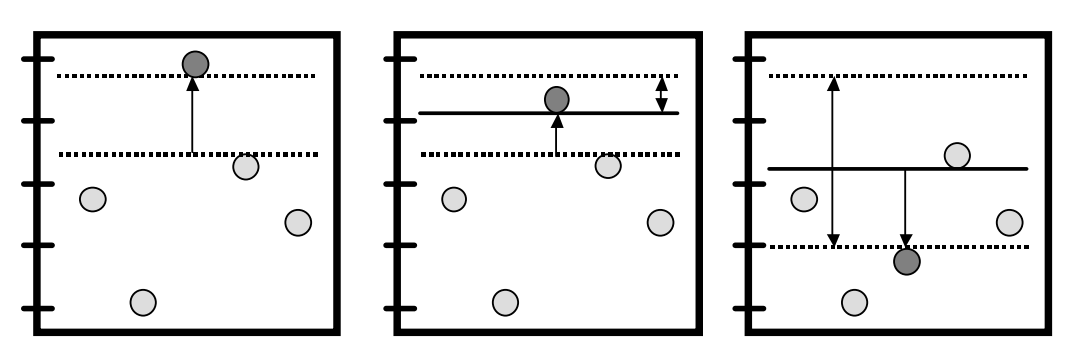
\includegraphics[scale=.5]{transfer/fig/svmloss.png}
	\caption{Illustration of the margin bound for a single example in 3 scenarios. The cirles denote different confidences and the correct label is ploted in dark grey. The height of each lable is the confidence score. In the left figure,$\epsilon(x)=0$. In the middle figure, even though the confidence of the correct label is the largest, it fails to be larger by 1 than the confidence of the runner-up and have a small loss. In the right figure, the confidence of the correct label is not the largest one and have a very large loss.}\label{fig:single:multi-loss}
\end{figure}

Let $\hat{y}_{ij}$ denotes the LOO-CV estimation of the example $x_i$ for binary model $f_i$. From Eq. \eqref{eq:single:looesti} we can see that:
\begin{equation}
\hat{y}_{ij} = y_{ij}-\frac{\alpha_{ji}}{\mathcal{S}^{-1}_{ii}}
\end{equation}
where the matrix $\boldsymbol{\alpha} = [\alpha_{ji}|i=1,...,l;j=1,...,N]$ should satisfy:
\begin{equation}
	\mathcal{S}\left[ {\begin{array}{*{20}{c}}
		\boldsymbol{\alpha} \\
		\boldsymbol{b}
		\end{array}} \right] = \left[ {\begin{array}{*{20}{c}}
		{Y - D(\gamma) X{{\left( {W'} \right)}^T}}\\
		0
		\end{array}} \right]
\end{equation}
Let:

\begin{equation}
\begin{array}{c}
{\mathcal{S}}\left[ {\begin{array}{*{20}{c}}
	{\boldsymbol{\alpha} '}\\
	{\boldsymbol{b}'}
	\end{array}} \right] = \left[ {\begin{array}{*{20}{c}}
	Y\\
	0
	\end{array}} \right]\\
{\mathcal{S}}\left[ {\begin{array}{*{20}{c}}
	{\boldsymbol{\alpha} ''}\\
	{\boldsymbol{b}''}
	\end{array}} \right] = \left[ {\begin{array}{*{20}{c}}
	{X{{\left( {W'} \right)}^T}}\\
	0
	\end{array}} \right]
\end{array}
\end{equation}
Thus we have:

\begin{equation}
	\alpha_{ji} = \alpha'_{ji} - \gamma_j \alpha''_{ji}
\end{equation}
The multi-class LOO-CV loss \eqref{eq:single:train_loss} can be re-written as:
\begin{equation}
	\begin{aligned}
	\epsilon^{(i)} _{multi} &= \mathop {\max }\limits_{n \in \left\lbrace 1,...,N \right\rbrace } {\left[ {1 - {\varepsilon _{n{y_i}}} + \hat{y}_{in} - \hat{y}_{iy_i}} \right]}\\
	&=\mathop {\max }\limits_{n \in \left\lbrace 1,...,N \right\rbrace }{\left[ {1 - {\varepsilon _{n{y_i}}} + {y}_{in}-\frac{\alpha'_{ni} - \gamma_n \alpha''_{ni}}{\mathcal{S}^{-1}_{ii}} - {y}_{iy_i}} + \frac{\alpha'_{y_ii} - \gamma_{y_i} \alpha''_{y_ii}}{\mathcal{S}^{-1}_{ii}} \right]}\\
	%&=\mathop {\max }\limits_{n \in \left\lbrace 1,...,N \right\rbrace }{\left[1-{\varepsilon _{n{y_i}}}\right]}
	\end{aligned}
\end{equation}
With the label encoding strategy in \eqref{eq:single:labelmatrix}, we the multi-class LOO error for example $(x_i,y_i)$ can be written as:
\begin{equation}
\epsilon^{(i)} _{multi} = \max \left(\mathop{\max}_{n \neq y_i}\left[\frac{(\alpha'_{iy_i}-\alpha'_{in})+(\gamma_n \alpha''_{ni}-\gamma_{y_i} \alpha''_{y_ii})}{\mathcal{S}^{-1}_{ii}}-2\right],0\right)
\end{equation} 
Thus the optimal transfer parameter $\gamma*$ should be the one that minimize the LOO-CV error $\epsilon _{multi}$ which is the average of the error for $\epsilon^{(i)} _{multi}$.

In summary, in this section, we introduce the multi-class loss for LOO-CV. We show that the multi-class LOO-CV loss is a function of the transfer parameter. Therefore, by finding the minimum of the multi-class LOO-CV loss, we can get the optimal transfer parameter.
